\chapter{はじめに}

\section{方針}

この教材は筑波大学生物資源学類1年次「物理学I」(奈佐原顕郎)の教材である。
まず, 本書の基本的な方針を示しておこう。

\begin{itemize}
\item 想定する学生は, 少なくとも高校の「数学IIIレベル」の数学力があり, かつ, 
中学理科の「1分野」を理解している人。高校「物理基礎」「物理学」は不問。
\item 副教材として生物資源学類の「数学リメディアル教材」を使う。
\item 物理学の理解に数学の学力は必須。「あったら良い」という程度でなく, 「必須」。
それも, 相当高度な数学が必要。この教材では, 前半部では主に「数学III」までの高校数学
を使うが, 後半部ではさらに大学の数学(微分方程式・偏微分・全微分・外積など)
も使う。これらの数学は「数学リメディアル教材」で自主的に学んで
おくこと。「とりあえず物理を勉強してみて, 数学が必要になったら
そのとき数学を勉強しよう」という考えは甘い!
\item 高校物理の履修は前提としないが, 一応, 高校物理の参考書として
山本・左巻「新しい高校物理の教科書」(講談社ブルーバックス)をお勧めする。
\item 物理実験の映像をたくさん見よう。物理学は机上の空論では
なく, 実際の自然現象を説明する理論だから, 実験を通して理解することが
絶対に必要。テレビ番組では以下がお勧め: 
\begin{itemize}
\item NHK教育「NHK高校講座 物理」\\...ネット上でも見れます。
\item NHK教育「ピタゴラスイッチ」\\...特にピタゴラ装置
\item NHK教育「大科学実験」
\item 日本テレビ「世界一受けたい授業」\\...特にでんじろう先生
\end{itemize}
他にも, ネット上(YouTubeなど)に, 良い動画がたくさんある。楽しんで見よう!
\item この教材の誤植訂正情報は, 以下のウェブサイトに掲載する:\\
http://ryuiki.agbi.tsukuba.ac.jp/lec/2017-physics/
\item この教材の内容は, (基本法則や慣習的に理解されていること以外は)全てオリジナルである。
ただし, Richard Feynman "Lectures on Physics" Addison-Wesleyから影響を
受けている(岩波書店から「ファインマン物理学」という題で和訳が出ている)。
\item ベクトルは, 細字や「文字に上矢印」ではなく, 太字で書くこと。
\item $x$を$\chi$と書かないように。
\item 数値を求める問題では, (無次元量でない限り)数値に単位をつけること。
数値の有効数字は, 特に指定がなければ, 2桁でよろしい。
\item 各章末に問題の解答を載せた。ただし一部の問題については解答を省略した
(「解答略」とすら載っていないものもある)。そのような問題は, テキストをしっかり
読めば自然に解答が見つかるはず。
\end{itemize}
\mv

\begin{faq}{\small\textgt{物理って必要なんですか? あんまり役立ち
そうな気がしないのですが} ... 物理は「役に立つ科学の
ナンバーワン」です。理系の学問で, 物理学のお世話になっていないものは
何一つありません。物理は空気と同じようなもので, 気にしなければ気づきま
せんが, 常に我々のまわりにある大切な存在です。}\end{faq}

\begin{faq}{\small\textgt{私は物理学は苦手だし、私の将来には
必要ないと思っていたのですが} ... ものごとの重要性や意味は, 
それを理解し習得した人にしかわからない, という面があります。
物理学を理解していない人は, 物理学は自分には不要だと思いがちです。
皆さんの先輩が「物理なんか必要ないよ」と言う場合, 多くは, その人
自身が物理を理解していないのです。でも, これから説明していきますが, 
どんな人にとっても物理学は役に立つ「お買い得」の学問ですよ。}\end{faq}

\begin{faq}{\small\textgt{物理って, 覚えた公式に数字を入れるだけ
じゃないのですか?} ... 大きな誤解です。物理学は実験事実と数学で
組み立てられる, 精密で普遍的な理論体系であり, 世の中のものの成り立ちや
現象の仕組みを根本から説明するスーパーパワーです。「公式に数字を入れる」
のは, 物理学のごく一部に過ぎません。}\end{faq}

\begin{faq}{\small\textgt{でも, ボールとかバネとか, ものの動き
をあれこれ考えるだけでしょ?}
 ... 「ものの動き」は物理学の対象のごく一部なのですが, 「ものの動き」が
わかるだけでも凄いことですよ。地震も津波も台風も「ものの動き」です。
化学反応も分子や原子という「ものの動き」です。魚が水中を泳ぐのも, 鳥が
空を飛ぶのも「ものの動き」です。高校物理で出てきたボールの軌跡や
バネの振動は, そのような森羅万象の「ものの動き」を説明する, 最初の
例にすぎません。}\end{faq}

\begin{faq}{\small\textgt{高校でやった物理基礎は面白くなかったのですが}
 ... 教科書に太字で記された公式を丸暗記して、単純な計算問題
を繰り返し解き, 解法のパターンを覚え、時間内に正確に多く解く, 
みたいな勉強をいくらやっても物理は楽しくなりません。物理の理論が
実際の現象にどのように対応するのかを自分の頭で考え, 
試し, 納得するまで自問自答する, という作業をすれば, 物理は面白く
なります。}\end{faq}

\begin{faq}{\small\textgt{物理, 嫌いです。どうすれば好きになれますか?} ... 
理解するまで考え抜くことと, 自分で試すこと。一方, やみくもに暗記とか, 
テストやレポートで点をもらうことだけにこだわると, 嫌いになります。}\end{faq}

\begin{faq}{\small\textgt{でも, テストやレポートで点がとれないと
成績が悪くなるし単位も貰えないじゃないですか。} ... 
成績や単位は, その学問を理解し, 習得したことの証明。ちゃんと
わかっていないのに良い成績をとろうとするのは「ごまかし」です。
そんな努力はあなたに何も残さないでしょう。}\end{faq}

\begin{faq}{\small\textgt{でも, 成績が悪かったり単位がとれないと, 就職や
進学で困ります} ... 仮に就職や進学でごまかせても, その後で
見抜かれますよ。最後に評価されるのは\underline{実力}だけです。}\end{faq}

\begin{faq}{\small\textgt{でも, やはり成績や単位が気になります}
 ... なら, 今のあなたにはこの授業は向いていないかもね。}\end{faq}

\begin{faq}{\small\textgt{高校で物理を勉強していないので不安です}
... あまり関係ありません。重要なのは高校数学と, 「わかろうとする執念」
です。この教材は, 高校物理未習だけど高校数III既習の学生を想定しています。}\end{faq}

\begin{faq}{\small\textgt{物理は高校で挫折しましたが, 高校数学
は学びました。リベンジできますかね?}
... 高校数学を修めた今こそ, 物理にチャレンジ&リベンジする時です! 
実際, 高校物理の難しさの大部分は, ちゃんと数学を使わない(文科省の
縛りで使っちゃいけないことになっている)ことにあります。ちゃんと数学を
使えば「覚えること」は半分以下に減り, 見通しもすっきりします。}\end{faq}

\begin{faq}{\small\textgt{このテキストは高校物理の復習ですか?}
... 高校物理と同じ題材も出てきますが, 高校物理では説明され
なかった(説明できなかった)部分を説明し, 理解していきます。
そのために数学をガンガン使います。「高校物理やったから簡単!」とか
思ってると痛い目にあいます。}\end{faq}

\begin{faq}{\small\textgt{私は高校物理既習ですが, 有利ではないのですか?}
... 高校物理をやった人は, 有利な面と不利な面があります。それぞれの題材
や問題に慣れ親しんでいるのは有利なこと。高校物理と似た話題を「それ
高校でやった」とスルーしてしまいがちで, 体系的な理解に到達しにくい
のは不利なこと。高校物理を忘れて, 謙虚にやりなおすことが何より大事。}\end{faq}

\begin{faq}{\small\textgt{てことは, もしかして高校物理をやったのは無意味?}
... そんなことありません。ただ, 人間は成功体験や先入観があると
新しいことを学びづらくなります。それに気をつけよう, と言ってるだけです。
謙虚にやり直せば, 「高校で学んだアレは実はこういうことだったのか!」
という驚きや感動が, 君を大いに成長させてくれるでしょうし, それは
高校で物理をやらなかった人には味わえない体験です。}\end{faq}

\begin{faq}{\small\textgt{簡単な公式は覚えておいた方が良いのでしょうか。} ... 
「公式」よりも, まず「基本法則」と「定義」をしっかり覚えましょう。
「公式」は, 基本法則と定義から論理的に導出されます。}\end{faq}

\begin{faq}{\small\textgt{質問は授業中よりも, 授業後に個別にするほうがいいですよね?} ... 
いえ! 授業中に, その場で質問して下さい!! その方が, 何倍もありがたいです。
「他の人の迷惑」とか「恥ずかしい」とか思わなくていいです。疑問をその場で
ぶつけてくれたら, あなただけでなく他の人たちにも説明できるし, 私の
ケアレスミスもその場で修正できます。}\end{faq}

\hv


\section{物理学とは}

自然現象は多種多様であり, それらの多くはどのように起きているのか
説明しがたいように思える。しかし, どんな自然現象でも少数の「法則」に
従うはずだと考え, そのような法則, すなわち「基本法則」\footnote{「基本原理」「第一原理」などとも言う。}
を解明し, 基本法則で自然現象を説明しようとする学問が物理学だ。

そして, そのような法則を見出すと, 執拗にその正しさを, あらゆる実験で
検証する。そして, その法則に合わない「例外」や「矛盾」を見つけたら, 
それをきちんと説明できて, かつ, もとの法則とも矛盾しないような, 
より包括的な基本法則を物理学は探す。そのとき武器になるのは数学だ。
物理学では, 人間の想像力が及ばない法則であっても, 数学の論理
と整合性は崩れないだろうと考え, 数学の力を信じる。だから, 
物理学には数学が必要なのだ。\mv

また, 物理学は, 全てのものごとを, それらの基本法則と数学だけで説明
しようとする。

例えば, 手に持ったボールを手放すと, ボールは地面に落ちるのはなぜだろう?

ありがちなのは「重力があるから」とか「地球がボールをひっぱてるから」という答である。
しかしこれは不十分である。仮に, 重力(地球がボールをひっぱる力)の存在は認める
としても, 地球がボールをひっぱるとなぜボールは落ちるのかが説明できていない。
そこで論理が飛躍しているのだ。「そんなの説明するまでもなくアタリマエのことだろう」
というのは, 物理学ではないのだ。

\begin{faq}{\small\textgt{なんか, アタリマエでどうでもいいことに
屁理屈というかイチャモンつけてるような気がしますが} ... 学問はそういうものです。
アタリマエのように思えることも疑ってかかって, きっちりした理論体系で「説明」
しようとするのです。}\end{faq}

まず, 質量を持っている物体同士にはたがいに引き合う力(重力)が働く, 
という基本法則がある(万有引力の法則)。地球もボールも「質量を持った物体」
なので, それらの間に力が働く。次に, 物体に力がかかると, 物体にはその力に
比例した加速度が生じる, という法則がある(運動の第二法則)。「ボールが地球
から受ける力」からボールの加速度を求め, それに数学(微積分学)を適用すると, 
物体の位置は地球に向かって移動する(落ちていく)ということが導き出される。
これが, 「ボールを手放したら地面に落ちる」ことの物理学的な説明である!\\

\begin{faq}{\small\textgt{それ, 説明になってます? 簡単なことをわざわざ難しく
言い換えてるだけのような気がしますが} ... いえ, そうではありません。このロジック
を使えば, 火星でもボールが落ちることを, そのスピードがどのくらいかも含めて
予測・説明できるし, 宇宙の彼方にある小惑星に探査機を飛ばして着陸し, 
地球に帰還させることもできるのです(「はやぶさ」)。そのような, 「行ったことのない
世界」の出来事まで, この物理学のロジックは予測・説明できるのです。}\end{faq}
\mv

\section{物理学の分野}

物理学の基礎は, おおまかに言って, 以下のような分野にわけられる:
\begin{itemize}
\item 力学\index{りきがく@力学}
\item 熱力学\index{ねつりきがく@熱力学}
\item 電磁気学\index{でんじきがく@電磁気学}
\item 相対論\index{そうたいろん@相対論}
\item 量子力学\index{りょうしりきがく@量子力学}
\end{itemize}

力学は「古典力学」\index{こてんりきがく@古典力学}とか「ニュートン力学」
\index{にゅーとんりきがく@ニュートン力学}ともいう。我々の日常的な時空間
スケールでの物体の運動を扱う。1学期に学ぶのはこの分野である。
津波の伝播, 地震波の伝播, 地球の周囲をまわる月の運動, 本田圭佑のフリーキック, 
浅田真央のトリプルアクセル, レインボーブリッジの強度や構造, 交通事故の衝撃等は, 
力学で解析できる。「運動の三法則」\index{うんどうのさんほうそく@運動の三法則}
と呼ばれる法則(慣性の法則・運動方程式・作用反作用の法則)が基本法則である。
万有引力\index{ばんゆういんりょくのほうそく@万有引力の法則}の法則も力学の一部である。
力学を数学的に洗練した「解析力学」\index{かいせきりきがく@解析力学}という分野もある。

熱力学は, 熱や温度が関与する現象を扱う。「化学I」や秋学期「物理学II」で
学ぶ。同じ対象を統計学の手法を使って解析する「統計力学」\index{とうけいりきがく@統計力学}
というのもあるが, 熱力学との区別は明瞭ではない。
そこで, 両者を一緒にして「熱力学」とか「熱・統計力学」と呼ぶこともある。
「熱力学の三法則」という法則(エネルギー保存則・エントロピー増大の法則・
絶対エントロピーの法則)が基本法則だ。多くの場合, 後述する量子力学
と組み合わさって威力を発揮する。気体の状態方程式(温度・圧力・体積の関係), 
比熱, 相転移(融解・蒸発等), 電池の活性などは熱力学で解析できる。地球温暖化
は大部分が熱力学の問題だ。

電磁気学は, 電気や磁気が関与する現象を扱う。「物理学II」の後半で学ぶ。
「マクスウェル方程式」というのがその基本法則だ。中学校以来なじみ深い
「オームの法則」は, 電磁気学と熱力学との境界に位置する法則である。身近な
電気製品はもちろん電磁気学の対象だ。分子や原子の間で働く力の大部分は
電磁気力なので, 物質の構造や性質を理解するためにも電磁気学は必要
だ。空間の電磁気的な性質が波として伝わる現象が「電磁波」すなわち「光」
だ。光を電磁気学的に解析する中で, 次に述べる相対論が生まれた。

相対論は, 大きな速さで運動する物体の運動に関する物理学である。電磁気学から
導かれ, 実験的にも確かめられたこととして, 光は誰から見ても一定の速さで飛ぶ, 
という事実がある。ここから出発し, 力学を修正したものを「特殊相対論」と呼ぶ。
その中で, 質量がエネルギーと同じものであることが示された。
また, 特殊相対論を包含し, さらに万有引力(重力)を説明するものを「一般
相対論」と呼ぶ。天文学には相対論が必要である。原子力(核反応)で解放される
エネルギーは相対論で説明される。カーナビで使うGPS (Global Positioning System; 
人工衛星からの電波によって, 地上の位置を高精度で計測するシステム)の
精度を高めるにも相対論が必要。

量子力学は「量子論」とも言う。主に原子や分子といった極微のスケールの現象
を説明する。「シュレーディンガー方程式」というのがよく出てくるが(秋学期の「化学II」でも
出てくるだろう), 必ずしもそれが基本法則ではない。量子力学の基本法則は
高度に抽象的で数学的だ。そこでは微積分だけでなく, 線形代数学(ベクトルや
行列の理論)や, 複素数, 確率などの考え方が活躍する。化学や生物学の
ミクロな現象は量子力学が支配する。光子が活躍する現象, 
例えば太陽光(熱放射)や, 植物の光合成, レーザー, 発光ダイオード(LED)
などは, 量子力学が無いと説明できない。コンピューター等の情報デバイス(半導体)
のほとんどは量子力学をもとに高性能化・小型化されている。病気や怪我をして
病院でMRI (核磁気共鳴画像法)の診断を受けた人もいるだろうが, あれは
物理学, 特に量子力学のカタマリである。筑波大学の前身だった
東京文理科大学で, 朝永振一郎教授がノーベル物理学賞をとったが, 
それは量子力学の一分野(量子電磁力学)を開いた功績によるものである。\mv

\begin{q}\label{q:basic_laws}
力学・熱力学・電磁気学の, それぞれの基本法則の名前を述べよ(内容はまだ理解しなくてよい)。
\end{q}
\vspace{0.2cm}

これらの物理学を組み合わせ, 発展させることで, 物理学は様々な対象を
扱う。宇宙論(天文学)や気象学, 多くの工学(電気工学・電子工学・建築工学・
土木工学・機械工学・航空工学・船舶工学)は, 物理学に立脚する(というか実質的
にほとんど物理学だ)。

一方で, 原子よりもずっと小さいスケールの粒子
(素粒子)の法則を追求し, 現有の様々な法則を統一的に理解するために「究極の法則」を
探す営為も, 物理学の先端で続けられている。湯川秀樹, 南部陽一郎, 益川敏英, 小林誠, 
小柴昌俊, 梶田隆章といった日本人物理学者がノーベル物理学賞を受賞したのは
この分野である。

また, その派生的な成果として, 様々な素粒子で人間の病気を治療する方法が
開発されたり(筑波大学病院の重粒子線治療), 火山の活動を素粒子で
透過的に観測する技術が開発されたりしている。

このように考えれば, ほとんどの科学は, 根本の部分で物理学に依存することが
わかるだろう。物理学以外の科学も多々あるが, それらが扱う対象は, ほとんど
が物理学の法則に従う。ただ, 往々にして対象が複雑・特殊過ぎて, 物理学の法則を
直接的に適用するのが大変だから, とりあえず物理学とは別の学問とするのだ。

そういうわけで, 「私は○○に興味があるから物理学は関係ない」という考え方は
とてもズレている。文化・経済・文学・芸術などですら物理学と無関係ではない。
文化や経済に大きな影響を与える新技術の開発や地球環境変動は, それを理解する
のに物理学が必要である。夏目漱石の小説には物理学の話題が多く登場する。
音楽は楽器の開発とともに発展したが, 楽器は非常に物理学的な装置(音響工学)である。\mv

\begin{faq}{\small\textgt{量子力学にとても興味があります。}
... この授業では量子力学についてほとんど言及できませんが, 量子力学は
すごい学問です。リチャード・ファインマン著「光と物質の不思議な理論」
(岩波書店)や, 朝永振一郎著「鏡の中の物理学」(講談社)などを読んで
みましょう。本格的に勉強したければ, 数学をしっかり勉強してください。}\end{faq}
\hv


\section{だまされないための物理学}

ところで, 世の中には, オカルト的な科学がたくさんある。物理学は, 
そのようなものへの耐性を君に与えてくれる。

\begin{exmpl} 「マイナスイオン」というのが健康に良い, という話が社会に
広まり, 「マイナスイオンを出す装置」なるものが開発・販売されている。
そういうのを聞いて, 懐疑的に思うのが物理学だ。物理学には
「電荷の保存則」という強い法則があり, それを否定する
実験結果は見つかっていない。もし「マイナスイオン」を発生するなら, 
それを打ち消すプラスの電荷がどこかにあるはずで, それはどこに
行っているのだ?
\end{exmpl}

\begin{exmpl}テレポーテーションやテレパシーという超能力に対しても, 
物理学は懐疑的である。物理学では, 「光よりも速く移動する物体
は無い」という強い法則(相対性理論)がある。それを
否定する事実を多くの物理学者が血眼になって探したが, 
いまだにひとつも見つかっていない。もし物体が瞬間的に
遠くに移動したら, その法則が崩れてしまう。\end{exmpl}

\begin{exmpl}水を凍らせる際に, 水にやさしい言葉をかけるときれいな氷の
結晶ができる, という話がある。これも物理学は懐疑的である。
物理学(熱力学)では, 物体の結晶成長に関する精密な理論
ができており, 結晶のできる様子は温度や圧力, 湿度(過飽和度), 
不純物の存在などによって決まることがわかっている。\end{exmpl}

\begin{exmpl}2003年頃, あるカルト宗教が「スカラー電磁波」なるものから身をまもる
ために, あらゆるものに白い布を巻き付けるという行動に出た
ことがテレビで報道されたが, 物理を学んだ人は, 
電磁波はベクトルの波であり, 「スカラー電磁波」などそもそも
存在しないと知っている。\end{exmpl}\mv

オカルト科学は, いかにも科学的な裏付けがありそうな言葉
で, 科学が苦手な人をだます。特に, 物理っぽい言葉がよく使われる
のは, 多くの人が物理が苦手だからだろうか。物理をきちんと理解していれば, 
オカルト科学にだまされる危険は大きく減るだろう。\mv

\begin{q}\label{q:fake_science} 社会を騒がせたオカルト的な科学
の例を1つ調べて, その概要と, 君ならそれをどう見破るかを
合計200字〜400字程度で述べよ。ただし, 上で例に挙げた事例はダメ。\end{q}
\hv


\section{ものづくりや研究のための物理学}
さて, 石だろうが紙だろうが生き物だろうが食べ物だろうが, 物を相手にする仕事には, 
測ったり作ったりということが不可欠になる。測るということは, 対象の特徴を, 数値的
な量に置き換えて表現することだ。その過程は物理学である。例えば溶液中
の化学物質の濃度を測るには, 特定の波長の光がその溶液をどれだけ透過するかを調べるが, 
その原理は物理学である。

原理を知らないでも, 説明書(マニュアル)のとおりにやれば, とりあえず計測機械を使うことは
できる。しかし, マニュアルを読みこなすには, 原理がわかっていないと大変だ。マニュアル
は人が書いたものなので, ミスもあり得る。あるいは「こんなことはマニュアルに書く
までもないだろう」ということもあるだろう。

実験したり物を作ったりするには, 計測だけでなく「制御」も重要になる。例えば生き物を育てるときに, 
温度や光, 湿度などの環境を一定に保つことは, しばしば必要になる。その原理も, 物理学である。
物理学をきちんとわかっていれば, 高価な恒温槽などを買わなくても手近な材料や機械を組み合わせて, 
適切な制御系を組むことができる。

このように, 計測も制御も, 多少なりとも機械が必要になる。機械は君の気持ちには無関係に, 
あくまでも物理学の法則に従って働くのだ。君が機械を手足のように自在に使いたいならば, 
機械の気持ち, つまりは物理学を理解しなければならない。そのためには, 物理学実験を学ぶ必要
がある。特に, 多くの機械は電気で動くから, 電気の知識は重要である。
\hv


\section{危機管理のための物理学}

さて, 社会にも人生にも危機(ピンチ)はある。生命を脅かすピンチの多くは物理的な現象である。
交通事故, 飛行機の墜落, 船の沈没などはニュートン力学(とその応用である流体力学)である。
特にこれから運転免許をとる諸君は, 車の構造や交通法規の背景に, たくさんの物理学
があることを意識しよう。意味や仕組みがわかってこそ, ルールも守る気になるものだし, 
結果的に安全な「カーライフ」を送ることにつながる。

自然災害 (津波や台風, 地震, 落雷, 火山噴火など)も, 多くは物理学(地球物理学)で扱われる。
落下や感電, 窒息なども物理現象である。これらを事前に予防したり, 対策したりするには, 
やはり物理学の考え方が重要だ。

家庭用電気製品は, 事故が起きないように, メーカーが慎重に設計・検証して作られる
ので, めったに事故は起きない。しかし, それでも老朽化すると故障するし, 
事故が起こる。それを防ぐのは, 個人の判断であり, 管理である。それには機械の動作原理の
理解, つまり物理学が必要である。

家電製品以外の機械, つまり研究・業務目的の機械は, 「プロ仕様」なので, 家電製品のような
徹底した安全対策や検証はされていないのが普通である。専門的な中小企業が作ることが
多いし品数が出ないので, そのような「素人向けの安全対策」までは手がまわらないのだ。従って, そのような
機械を扱うときには, 慎重さと判断力, 熟練が必要で, それが, 多くの資格が必要な理由である。
そういう資格試験の問題の多くは物理学である。
\hv


\section{スポーツや音楽のための物理学}

意識している人は少ないが, 実は, スポーツと音楽は物理学のカタマリである。
テニスで速いサーブを打つには? サッカーでボールのスピードを上げるために
芝に水を撒くのはなぜ? 相撲で小さな力士が大きな相手に押し負けられない
ようにするには? などなど, 多くの工夫やスキルは, 物理学の観点で
裏付けできるし説明できる。だからスポーツ用品メーカーの開発部はまるで物理学の
研究室だ。物理学がわかると, 他人のフォームやスキルの中の良いところ
に気付きやすくなるし, 自分の癖に気付いたり人からのアドバイスを理解したり
もスムーズになる。\mv

良い音色を出す楽器の構造は? 気温や湿度で楽器のチューニングが
狂うのはなぜ? 良い音でレコーディングするにはどんな工夫が
必要? 野外ライブでは電源をどのように確保・配給すればいい? ノイズを
カットするにはどういうことに気をつけて配線すべき? 音階が狂うのはなぜ? 
などなども物理学で説明できる。だから音楽をやる人は, 物理学を学んで
損は無い。\hv

\section{生物資源学類と物理学}

生物資源学類生の中には, 「自分は生物学に興味があるので物理学
は不要だ」とか思っている人もいるが, そういう考え方は間違っている。
生き物の機能や構造がどのように作られているのかを理解するには
物理学は必須だ。昆虫が固い殻(外骨格)を持っていることには, 
物理学的な理由がある。魚が高速で水中を泳いだり, 鳥が空を飛ぶ
のは, 彼らが物理学的に合理的な身体構造と機能を持っている
からだ。植物は光合成で獲得した炭素を, 根・幹・葉・生殖器官に最適に
分配しているが, その戦略は, 物理学的な事情(根から水を効率的に吸い上げる・
風などの外力で倒れたり折れたりしない・多くの光を葉に受ける・種子を風に
乗せて遠くに飛ばすなど)で決まる。

農業の効率化に灌漑施設や農業施設, 農業機械は不可欠だが, それらを低コストで
効率よく働かせるには, 物理的に最適な設計と配置が必要だ。田畑に霜が
おりると作物はダメになってしまうので, 霜がおりないような工夫をするのだが
(茶畑で扇風機がくるくるまわってるやつとか), それも物理学だ。乾燥地農業
で塩類集積が問題になるが, あれを予測・制御するには土壌水分と塩類の
移動を物理学でモデル化する必要がある。家畜が逃げないように牧場のまわりに
電気柵を張り巡らすが, それを安全に扱うには電気の知識(結局は物理学)
が必要だ。地域で伝統的に行われている
農法や漁法(霞ヶ浦の帆引き船など)には, 物理学的に理にかなった工夫
が随所にある。そういうのを理解しないと, 伝統の継承や発展は難しい。

地球環境を保全するには, 人工衛星で地球を観測する必要があるが, そこで
は衛星の軌道制御や観測装置の設計などで, 膨大な物理学的知識
が使われている。土砂災害を防ぐには, 地すべりや土石流の発生と移動を
予測し制御する必要があるが, その中心は物理学だ。物理学を駆使して, 
起き得る災害を正確に予測できれば, コンパクトで効率的なダムや堤防
を作ることができ, 経費の節約や環境保全になる。

食品の保存や加工, 微生物の培養などには, 最適な温度・湿度環境が必要
だが, その制御には物理学が活躍している。
\hv

\section{科学者・技術者としての一生の基礎を作ろう}

以上のように, 物理学は, ほとんどありとあらゆる場面に登場する。
しかし, 仕事や研究の個々の場面では, 物理学の法則まで
わざわざ立ち返って検討したりしなくても, 既にマニュアルや
ノウハウや慣例が存在し, それに従っていれば問題なく
やりすごせるものである。そこで、若い人の多くは, 「物理学なんか
学ぶよりも, 実用的な技術を身につける方が楽だし意味がある」
と思うものである。

ところが, そういう人も, 歳をとってくると, 不思議なことに, 
「ああ, 若い時に物理学をちゃんと理解しておけばよかった...」
と後悔し, 嘆くものである。とりわけ, 多くの立派な仕事をこなしている
プロフェッショナルな人ほどそのように言うのだ(だから, 
「物理学なんかやっても仕方ないよ」と君に言う大人は, プロ
として甘い仕事をしている人である可能性がある)。

科学や技術の進歩は速い。若い時に身につけた技術も
やがて陳腐化する。諸君は歳をとっても, 多くの新しい技術を身に
つけねばならなくなる。仕事や研究の現場で, まだマニュアルや
ノウハウになっていない問題や矛盾に出会うこともある。
そういうときに役立つのが, 物理学を含む, 基礎科学なのだ。

基礎科学は, ビルディングの壁の中に埋められた鉄骨のような
ものである。普段はその存在は見えないし, 意識されることも無い。
しかし, そのビルディングを地震や強風, 洪水や津波が襲った
とき, 最後に頼りになるのがそれらである。順風満帆で「普段通り」
が続く日常では物理学をことさら意識しないでもなんとかなるが, 
人生はそんなに甘くない。
\hv


\section{法則・原理・定義・公理・定理}

ここで, 法則\index{ほうそく@法則}・原理・定義・公理・定理などの言葉の意味を確認しておこう。

\begin{itemize}
\item 法則 ... 自然現象や社会現象の中に見られるルール。物理学・化学・
生物学・経済学などで使う。数学ではほとんど使わない。例:万有引力の法則
\vspace{0.1cm}
\item 原理\index{げんり@原理} ... 法則と同じようなもの。ただし, 法則の中でも, より根源的
なもの(基本法則に近いもの)を原理と呼ぶ傾向がある。例:アルキメデスの原理
\vspace{0.1cm}
\item 定義\index{ていぎ@定義} ... 言葉の意味を定めること。
\vspace{0.1cm}
\item 公理\index{こうり@公理} ... 定義と同じようなもの。主に数学で使う。言葉の意味を定める
だけでなく, そのようなものが存在することを認めよう, という立場も示す。
例:ユークリッド幾何学の公理
\vspace{0.1cm}
\item 定理\index{ていり@定理} ... 公理や他の定理から論理的に導かれること。主に数学で使う。
定理の中で, いまいち影が薄いものを, 補題と呼ぶ。例:三平方の定理
\end{itemize}

法則Aと法則Bがあって, 法則Aで説明できることはすべて法則Bでも説明され, 
なおかつ, 法則Aでは説明できないが法則Bで説明できるようなこともあるような
場合, 法則Bは法則Aより\textgt{一般性が高い}, という。そのような場合は, たいてい, 
法則Aは法則Bの特別なケースであり, 法則Bから法則Aを論理的に導出すること
ができる\footnote{ところが, 科学というのはおもしろいもので, 法則Bから
論理的に導かれる法則Aのほうが一般性が高いということも, たまにある。例えば
「力学的エネルギー保存則」という法則は運動の三法則から導かれるが, 
「エネルギー保存則」は力学の範囲を超えて普遍的に成り立つ法則でもある。}。

科学は, より一般性の高い法則を見出すことを目指す。最も一般性の高い法則
(つまり根源的な法則)を「基本法則」\index{きほんほうそく@基本法則}とか
「第一原理」\index{だいいちげんり@第一原理}と呼ぶ。しかし, 基本法則は
抽象的なので, 実際には使いづらいこともある。そこで, 具体的によくある状況
に限定して基本法則を変形することで, 「適用範囲は狭いが扱いは簡単」な法則
が生まれる。しかし, その手の法則は無数にあって, きりがない。それに, 
それぞれの「適用範囲」を覚えて判断するのが面倒くさい。

例えば, 一定の力を受けて直線上を動く点の位置や速度を表す法則
(というか公式)がある(高校物理を習った人なら覚えているだろう, 
$x=x_0+v_0t+\frac{1}{2}at^2$というやつだ)。この法則は, 
力が変化する状況では成立しない。それがなぜなのか, とか, その
代わりに何を使えばよいのか, などを理解するには, 運動方程式
という基本法則と, それを記述する数学(微積分学)に戻らないとダメである。

君は, 多くの法則をばらばらに覚えるのではなく, 何が基本法則で, そこから
どのような条件でどのような派生法則が生じるのか, といった体系性を意識して学ぼう。\mv

ところで, 「オッカムの剃刀\footnote{剃刀は「カミソリ」と読む。}」
\index{おっかむのかみそり@オッカムの剃刀}という考え方がある。基本法則として, 複数の候補があった
とき, それらが同程度に有効であるなら, より単純なほうが正しい, という考え方である。
これは必ずしも常に正しい考え方とは言えないが, 物理学(と多くの科学)は「無矛盾さ」
の次に「シンプルさ」を求める傾向にある, ということは覚えておこう。\mv

\begin{q}\label{q:OccamsRazor}
オッカムの剃刀とは何か?
\end{q}
\hv



\section{概算}
いろんな自然現象や社会問題について, 具体的な数値をもとに定量的に考えることに, 
あまり慣れていない人も多いだろう。しかし, 問題を「数」として量的に把握することは, 
とても大切である。\mv

基本的ないくつかの数字と, 各分野における基本法則, そして常識と少しの数学(特に対数や近似)
を使いこなすことで, 多くのことを「おおざっぱ」に「ざっくり」と見積り, 理解できる。
これは, 普通はほとんど教育されることはないが, とても重要なことである。\mv

たとえば,現在, 日本政府の債務(赤字, つまり借金)の額は, 約1000兆円である。
15桁にもおよぶ金額だが, 多くの国民にとって, まず重要なのは, その15桁の
全ての数字なのではなく, 15桁という桁数, すなわち「規模」である。

ところが多くの人は「1000兆円なんて大きすぎてピンと来ない」と言う。高等教育を
受ける人がそんなことを言ってはならない。想像しにくい規模の数を想像するには, 
「〜〜あたり」という視点に立てば良い。膨大な額の借金も, 国民のひとりあたりの
借金に換算すれば, 想像しやすくなるだろう。日本の人口は約1億人だから, 1000兆円
÷1億人で, 1000万円/人, つまりひとりあたり1000万円である\footnote{信じられない, 
奈佐原はまた誤植をしているのではないか? と思う人は, 自分で調べてみたらよい。}。
こんな調子で, 「だいたい」でいいから, 何らかの数値をぱっと出すことを, 
概算\index{がいさん@概算}という。

\begin{faq}{\small\textgt{概算はどこまでアバウトでいいのですか?}
... 一概には言えませんが, ±50パーセント程度でいいのでは。}\end{faq}\mv

\begin{q}\label{q:soccer}
ある人の息子が, 「僕は将来, サッカー選手になりたい」と言う。その夢を応援
するためには, 親としては, それがどれだけ厳しい戦いになるかを知っておかねばなるまい。
\begin{enumerate}
\item 日本のサッカーのプロリーグ(Jリーグ; J1, J2, J3をあわせて)には, 
約50チームがある。各チームに選手は30人いるとして, 日本のプロサッカー選手の人数を概算せよ。
\item サッカー選手の選手寿命は短い。平均5年で引退すると考えて, Jリーグで1年間に
引退するサッカー選手の総数を概算せよ。それが, 1年間に新たにサッカー選手になれる人数だろう。
\item 一方, 小学校1学年には, 何人の男の子がいるだろうか? 少子化とかは無視して, 
日本の人口を1億人, 平均寿命を100年として概算せよ。
\item 一学年の男子のうち, 何人に一人が, 夢をかなえてサッカー選手になれるのだろうか? 
\end{enumerate}
\end{q}
\mv

\begin{q}\label{q:Japan_debt}
2016年現在, 日本の年間の国家予算は約100兆円である。また, 日本から国際連合
(国連)への年間の拠出金額は約250億円である。これらの数字を, (1) 政府の借金に比べて
どのくらいの大きさか?  (2) 国民ひとりあたりいくらか? という, 2つの観点で, 概算で
評価せよ。有効数字は1〜2桁でよい。
\end{q}
\vspace{0.2cm}

\begin{q}\label{q:Japan_rain_paddy}
日本の平均年間降水量は1500~mm程度である。一方, 日本では, 水田1 m$^2$あたり, 500~g
程度の米がとれる。一方, 米1~kgの生産には3000~kgの水が必要とされる。日本では, 水田に
降る雨だけで, この水量をまかなうことはできるか?
\end{q}
\hv



\section{質点モデル}

我々はこれから, 力と物体の運動に関する法則を学ぶのだが, まず, 
「質量」という概念を受け入れよう。質量とは, 物体の根源的な
属性(物体を特徴付ける性質)のひとつであり, 「どうやらそういう
ものが存在するらしい」と受け入れるしかない。質量とは何か, 質量はなぜ
存在するのか, ということを執拗に探求する物理学者達の熱い戦いは
まだ続いているが, とりあえずそれは彼らに任せて, 我々は
先に進む。感覚的には, 質量は物体の重さとか物体の「動かしにくさ」
に関係するような性質である。\mv

次に, 「質点」\index{しつてん@質点}という概念を定義しよう: 
質点とは, 質量は持つが大きさは持たない, 点状の仮想的(理想的)
な物体である。

現実の物体は大きさや形を持つのだが, 大きさや形を考えると, 物体に働く力
がややこしくなるのだ。例えば, 大きな物体の各部位に働く力がまちまちだったりすると, 
物体全体に働く力はもうわけがわからぬ, ということになる。そこでとりあえず, 
質点とみなせるくらい小さな物体に働く力を考える。そうやってひとまず大きさや
形といった属性を切り捨てることで, 次節以降に述べる諸々の力の法則や, いずれ
学ぶ「運動の三法則」という単純かつ強力な法則を見出すことができたのだ。

このように, 現実のものや現象を単純化・抽象化してとらえ直し, 扱いやすく
した近似的概念を「モデル」(模型)\index{もでる@モデル}と呼ぶ。質点は, 
物体のひとつのモデルである。

なら「質点」は空想の産物, 机上の空論に過ぎないのかというと, そうでもない。
現実の中には, 物体の大きさや形を近似的に無視できるような現象がたくさんあり, 
そのような場面では, 質点の議論がほとんどそのまま成り立つ。物体の大きさや形
が無視できなくても, 質点としての考察は議論の出発点として役立つことが多い。

\begin{exmpl} 野球のボールは, ある場合は質点とみなせる。例えば, ボールを
初速度100~km/hで斜め45度の角度で地上から空に投げる時, どこまで遠く飛ぶか?
のような問題では, ボールは質点と考えてモデル化しても, ほぼ差し支えない。
\end{exmpl}

どうしても大きさや形を考慮しないとまずい状況では, 質点の集合
(それを質点系という)として物体をモデル化するのである。そうして, 質点の理論
に持ち込むのである\footnote{その場合は, 後述するように, 角運動量や
慣性モーメントといった概念が必要になる。}(図\ref{fig:particle})。\mv

\begin{exmpl} 野球のボールは, 微妙な運動, 特にボールの回転が重要で
あるような運動では, 質点とみなしてはダメである。例えば, カーブやシュート
などの変化球は, ボールが回転することで周囲の空気に乱れを生じさせ, 
それによってボールが受ける力が変化することで起きるため, ボールの形・
大きさを無視できない。このような場合は, ボールは質点系としてモデル化すべきである。
\end{exmpl}

\begin{figure}[h]
    \centering
    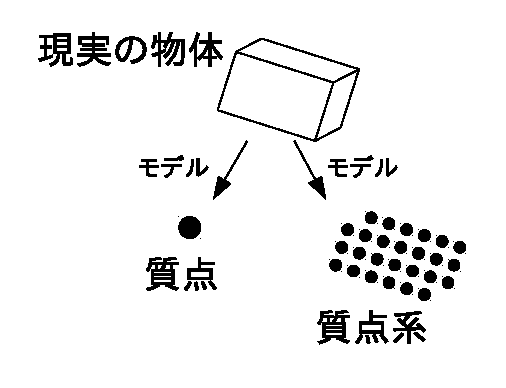
\includegraphics[width=5cm]{particle.eps}
    \caption{物体のモデル。大きさと形を無視できる場合は質点。そうでない
場合は質点系としてモデル化する(質点系では質点どうしの間に働く力も考える。
そうすることで物体がバラバラにならないように理論化できる)。}\label{fig:particle}
\end{figure}

\begin{q}\label{q:whatis_model}
モデルとは何か?
\end{q}

\begin{q}\label{q:whatis_particle}
質点とは何か?
\end{q}

モデルは科学のあらゆるところにある。例えば化学でいずれ学ぶ「理想気体」は現実
の気体のモデルのひとつである。

現実の現象や物体は往々にして複雑だが, それを複雑なままで見ているだけでは, 
仕組みはわからない。人間のしょぼい知性では複雑なものを理解できないのだ。
しかし複雑さをばっさり切り捨てて, 単純な状況に限定すると, 自然の仕組み
は人間ごときにも理解できることがある。だからモデルが必要なのだ。モデルの
力を借りて科学は進歩してきた。

ところが, いったん出来上がった科学を学ぶ我々は, 恩あるモデルの存在を忘れ, 
モデルに限って成り立つ法則が, 現実の複雑な現象にそのまま全面的に成り立つような
錯覚を起こしがちである。これは大変危険なことである。

\begin{exmpl} 君は小学校
で振り子を習っただろう。そこで振り子の周期は振れ幅に依存しない, と習った
はずだ。これを振り子の等時性\index{とうじせい@等時性}という。ところが, 
振り子の等時性は, 振り子の振れの角が十分に小さいという単純なモデルについてのみ成り立つ
近似的・限定的な性質である。振れの角が大きくなれば, 等時性は成り立たない。
実際, 振れの角が60度になれば周期は7パーセント程度長くなる
ことがわかっている。ちなみにこの「ずれ」は, 物理学と数学の理論で説明できる。
\end{exmpl}

君はこれから学ぶ科学の様々な事柄に対して, それがどのような限定の
中で成り立つかを注意深く理解しなければならない。そのためには, 
法則や理論の結論だけを丸飲みするのではなく, その理論の成立する
過程をきちんと理解し, それが現実の中の何をモデル化しているのか
理解しなければならない。
\hv



\begin{exq} 「筑波大学ギャラリー」(大学会館の中にある)を訪れて, 筑波大学にゆかりの
あるノーベル物理学賞受賞者に関する展示物の中から, あなたにとって最もインパクトの
あったものを報告せよ(その理由も含めて)。\end{exq}

\begin{exq} エンジニアや科学者にならない人も物理学を学ぶべきだろうか? 
君の考えを論じよ。\end{exq}


\section*{解答}

以下, 解答が無い問題は, 解答が略されているものである。\\

\noindent{\textbf{答}}\ref{q:basic_laws}\\
力学の基本法則: 慣性の法則・運動方程式・作用反作用の法則。万有引力の法則を加えることもある。
熱力学の三法則: 熱力学第1法則(エネルギー保存則)・熱力学第2法則(エントロピー増大の法則)・
熱力学第3法則(絶対エントロピーの法則)。
電磁気学の基本法則: マクスウェル方程式\footnote{それぞれの基本法則は, 別の形で言い換えることも
できる。特に, 熱力学第2法則やマクスウェル方程式の一部は, 別の形や名前で表現されることがある。}。
\vspace{0.2cm}

%\noindent{\textbf{答}}\ref{q:fake_science} 略
%\mv

% オッカムの剃刀とは何か?
\noindent{\textbf{答}}\ref{q:OccamsRazor}\\
基本法則として, 複数の候補があったとき, それらが同程度に有効であるなら, 
より単純なほうが正しいだろう, という考え方
\vspace{0.2cm}

% ある人の息子が, 「僕は将来, サッカー選手になりたい」と言う。
%\noindent{\textbf{答}}\ref{q:soccer}
%\begin{enumerate}
%\item $30\times30$で, 約1000人。正確には1067人だそうです(2010年Jリーグ発表)。
%\item $1000/5$で約200人。
%\item 1学年の児童は$100000000/100$で約100万人。このうち男子が半分として50万人。
%\item 200/50万で, 約0.0004。つまり1万人に4人, つまり2, 3千人にひとり。
%\end{enumerate}
%\vspace{0.2cm}

% 2011年現在, 日本の年間の国家予算は約100兆円である。
%\noindent{\textbf{答}}\ref{q:Japan_debt}
%\begin{enumerate}
%\item 年間国家予算は全借金の1/10程度。年間国連拠出金は全借金の1/40000程度。
%\item 年間国家予算はひとりあたり100万円程度。年間国連拠出金はひとりあたり250円程度。
%\end{enumerate}
%\vspace{0.2cm}

% 日本の平均年間降水量は1500mm程度である。
\noindent{\textbf{答}}\ref{q:Japan_rain_paddy}\\
日本の水田に, 1~m$^2$あたり1年間に必要な水量は, 0.5~kg$\times$3000~kg/kg=1500~kg。
水の密度は約1000 kg/m$^3$だから, これは1.5 m$^3$に相当。これを面積 1~m$^2$の地平面に
敷くと, 厚さは1.5~m, つまり1500~mmになる。一方, 日本の平均年間降水量は, 1500~mmなので, 
なんとか雨だけで足りる(計算上は)\footnote{現実は, もっと難しいことがいっぱいあるので, 
ほとんどの水田で灌漑が必要です。}。
\vspace{0.2cm}

% モデルとは何か?
%\noindent{\textbf{答}}\ref{q:whatis_model}
%現実のものや現象を単純化・抽象化してとらえ直し, 扱いやすくした近似的概念。
%\vspace{0.2cm}

% 質点とは何か?
%\noindent{\textbf{答}}\ref{q:whatis_particle}
%物体のモデルのひとつであり, 質量は持つが大きさは持たない, 点状の仮想的(理想的)な物体。
%\hv
